\subsection{Estimation of \texorpdfstring{$\tau_{\min}$}{tau-min}}
\label{sec:reach}

    If $M$ has reach $\tau$, then at least one
  of the following cases holds:
\begin{enumerate}
	\item[I] (Global case) $M$ has a bottleneck, i.e. there exist $p, q \in M$, such that $(p+q)/2 \in \text{Med}(M)$ and $\|p-q\|=2\tau$.
	\item[II] (Local case) There exists $p \in M$, and an arc-length parametrized geodesic $\gamma$ such that $\gamma(0)=p$ and $|\gamma^{\prime\prime}(0)|=1/\tau$.
\end{enumerate}
where $\text{Med}(M)=\left\{z\in \mathbb{R}^D: \exists p\neq q\in M, \|z-p\|=\|z-q\|=d_E(z,M) \right\}$, $d_E(x,M)$ is the distance between $x$ and $M$.

We denote global reach and local reach as $\tau_g$ and $\tau_l$, respectively. Thus $\tau = \min \left\{\tau_g, \tau_l\right\}$

\begin{figure}[H]
	\centering
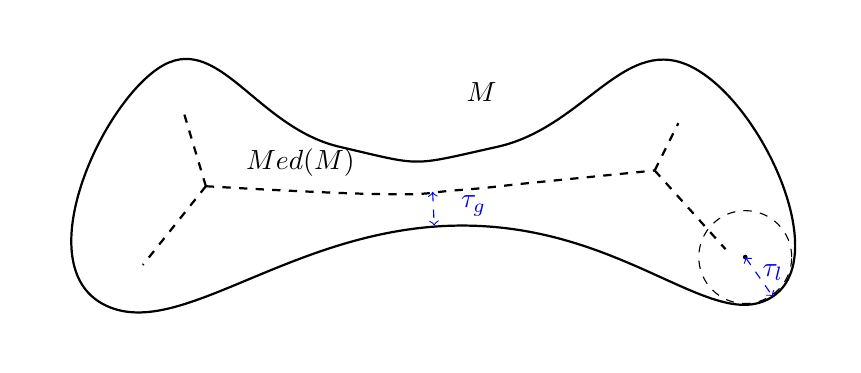
\begin{tikzpicture}
	
	% 绘制M的不规则形状
	\draw[thick] plot [smooth cycle, tension=0.9] coordinates {(-4.5,-1.5) (-3.8,1.5) (-1.5,0.5) (0.5,0.5) (3,1.5) (4,-1.4) (0,-0.5) };
	\draw[dashed] (3.65,-0.9) circle [radius=0.59];
	\fill (3.65,-0.9) circle [radius=0.03];
	\draw[<->, dashed, blue] (3.65,-0.9) -- (4,-1.4);
	
	\node[blue]  at (4.0,-1.1) {\(\tau_l\)};
	% 绘制中轴线Med(M)
	\draw[dashed, thick] plot [smooth, tension=0.8] coordinates {(-3.2,0) (-1,-0.1) (0,-0.05) (1,0.05) (2.5,0.2)};
	
	% 绘制两端的分叉
	\draw[dashed, thick] (-3.2,0) -- (-4,-1);
	\draw[dashed, thick] (-3.2,0) -- (-3.5,1);
	\draw[dashed, thick] (2.5,0.2) -- (3.4,-0.8);
	\draw[dashed, thick] (2.5,0.2) -- (2.8,0.8);
	
	% 绘制TM距离的箭头
	\draw[<->, dashed, blue] (-0.32,-0.07) -- (-0.3,-0.5);
	
	% 标注文字
	\node[blue] at (0.2,-0.25) {\(\tau_g\)};
	\node at (0.3,1.2) {\(M\)};
	\node at (-2,0.3) {\(Med(M)\)};
	
\end{tikzpicture}
	\caption{Reach}
\end{figure}

We can define $\tau_l$ easily by 
\begin{align}
	\tau_l := \inf\limits_{p\in M} \left\{\frac{1}{\|\mathrm{II}_p\|}\right\}.
\end{align}

We will show that there exists a uniform positive lower bound on the reach of $\varphi(M)$ for all $\varphi(M) \in \varphi(\MM)$:
\begin{theorem}[Uniform lower bound on the reach of $\varphi(\MM)$]
	\label{thm:reach-bound}
	There exists a positive constant $\tau_{\varphi(\MM)}$, depending only on the uniform geometric parameters of $\MM$ and on the DM parameters $(m,t_0)$, such that
	\begin{align}
		\tau_{\varphi(M)} \geq \tau_{\varphi(\MM)} > 0 \qquad \text{for all } M \in \MM.
	\end{align}
\end{theorem}
The bound is obtained by writing $\tau = \min\{\tau_l,\tau_g\}$ and bounding each term separately: the local reach is controlled through the second fundamental form of $\varphi(M)$ (\cref{lem:local-reach}), and the global reach is controlled in \cref{sec:glo-reach}.







%%% Using geodesic curvature

\iffalse
%now we prove in normal coordinate chart of $M$, $|\frac{\partial f_i}{\partial x_k}|$ and $|\frac{\partial^2 f_i}{\partial x_k \partial x_p}|$ are bounded. We consider a curve $(tv^1,tv^2,...,tv^d) \subset \hat{U}$, then $(f_1(tv^1,tv^2,...,tv^d),...,f_D(tv^1,tv^2,...,tv^d))$ is the geodesic starting at $p$ with initial velocity $v^i\partial_i(p) \in T_pM$. We take $v^k=1$ and others equal $0$, then $(\frac{\partial f_1}{\partial x_k},...,\frac{\partial f_D}{\partial x_k})(0,...,t,...,0)$ is the unit tangent vector along this geodesic， thus $|\frac{\partial f_i}{\partial x_k}|\leq 1$. We take second order derivative, and use the assumption $|\gamma^{\prime \prime}(s)|$ is bounded, we obtain $|\frac{\partial^2 f_i}{\partial x_k^2}|$ is also bounded. If we ask $v^k= v^p = \frac{\sqrt{2}}{2}$ and take second order derivative, we have $|\frac{\partial^2 f_i}{\partial x_k^2}+2\frac{\partial^2 f_i}{\partial x_k\partial x_p}+\frac{\partial^2 f_i}{\partial x_p^2}|$ is bounded, since $|\frac{\partial^2 f_i}{\partial x_k^2}|$ is bounded, by triangle inequality, $|\frac{\partial^2 f_i}{\partial x_k \partial x_p}|$ is bounded


Using tangent vector, we obtain the metric tensor, whose $(i,j)$ component is 
\begin{align}
	g_{ij}=\left\langle r_i,r_j\right\rangle 
\end{align}
we take partial derivative of it, we have 
\begin{align}
	\frac{\partial g_{ij}}{\partial x_k}=\left\langle r_i , \frac{\partial r_j}{\partial x_k}\right\rangle + \left\langle \frac{\partial r_i}{\partial x_k} , r_j\right\rangle 
\end{align}
we have proved $|\frac{\partial^2  \varphi_i}{\partial x_k \partial x_p}|$ and $|\frac{\partial \varphi_i}{\partial x_k}|$ are bounded, so $\frac{\partial g_{ij}}{\partial x_k}$ is bounded since both $r_i$ and $\frac{\partial r_j}{\partial x_k}$ are bounded.

The Christoffel symbol is 
\begin{align}
	\Gamma^\lambda_{\mu\nu} = \frac{1}{2} g^{\lambda\sigma} \left( \frac{\partial g_{\sigma\nu}}{\partial x^\mu} + \frac{\partial g_{\sigma\mu}}{\partial x^\nu} - \frac{\partial g_{\mu\nu}}{\partial x^\sigma} \right)
\end{align}
where $g^{\lambda \sigma}$ is the inverse matrix of $g_{ij}$, so $g^{\lambda \sigma}=\frac{1}{det(g)} det(C_{\lambda \sigma})$ is also bounded, where $C_{\lambda \sigma}$ is the $(\lambda, \sigma)$ cofactor. Now we consider the lower bound of $det(g)$, we have
\begin{align}
	g_{ij}=\left\langle r_i,r_j\right\rangle = \sum_{k=1}^m \frac{\partial \hat{\varphi}_k}{\partial x_i} \frac{\partial \hat{\varphi}_k}{\partial x_j}
\end{align}
thus $g=J^T J$, where $J=\left(\frac{\partial \hat{\varphi}_i}{\partial x_j}\right)\ i=1,\dots,m, \ j=1,\dots,d
$. We have proved the eigenvalues of $J^TJ$ is close to $1$, so $det(g)= det(J^TJ)$ is bounded below. Therefore, Christoffel symbols are bounded uniformly.




We consider a geodesic $\gamma(t)$ passing through $\varphi(p) \in V \subset \varphi(M)$, its coordinate representation is $(z_1(t),\dots,z_d(t))$. According to geodesic equation, we have 
\begin{align}
	\frac{d^2 z_k}{dt^2}+\Gamma_{ij}^k\frac{dz_i}{dt}\frac{dz_j}{dt}=0, \quad k=1,2,\dots,d
\end{align}

$\dot{z}(0)=(\frac{dz_1}{dt}(0),\dots,\frac{dz_d}{dt}(0))$ is the velocity of $z(t)$ in $\mathbb{R}^d$, by property of exponential map, the velocity at $p$ of $\textbf{x}^{-1}(z(t))$ is also $\dot{z}(0)$, thus $d\varphi_p \dot{z}(0)$ is the velocity of $\gamma(t)$, whose norm is $1$. Since $\|d \varphi\|>1-\epsilon$, $|\dot{z}(0)|<1/1-\epsilon$. Therefore $\frac{dz_i}{dt}$ is bounded, thus $\frac{d^2 z_i}{dt^2}$ is also bounded. 



%If we assume coordinate chart $(U,f)$ can control norm of tangent vector, in additon, $\|d\varphi\|$ is close to $1$. We derive $\frac{dz_i}{dt}$ is bounded, thus $\frac{d^2 z_i}{dt^2}$ is also bounded. 

The coordinate of $\gamma(t)$ in $\varphi(M)$ is $\gamma(t)=\left(\hat{\varphi}_1(z_1(t),\dots,z_d(t)),\dots,\hat{\varphi}_m(z_1(t),\dots,z_d(t))\right)$, we can obtain the second order derivative of $\gamma(t)$, its $p$-th component is
\begin{align}
	\gamma^{\prime \prime}_p=\frac{\partial^2 \hat{\varphi}_p}{\partial x_i \partial x_j}\frac{dz_i}{dt}\frac{dz_j}{dt}+\frac{\partial \hat{\varphi}_p}{\partial x_i}\frac{d^2z_i}{dt^2}
\end{align}
which is bounded, thus $|\gamma^{\prime \prime}(0)|$ is also bounded. $p$ and $\gamma(t)$ are arbitrary, $|\gamma^{\prime \prime}(s)|$ are bounded above. Therefore, $\tau_l$ of $\varphi(\mathcal{M})$ is bounded below by $c(\MM)$ which is depending on geometric setting of $\MM$.
\fi






